\documentclass{standalone}
\usepackage{tikz}
\usetikzlibrary{patterns, positioning}
\usepackage[sfdefault]{ClearSans} %% option 'sfdefault' activates Clear Sans as the default text font
\usepackage[T1]{fontenc}

\begin{document}
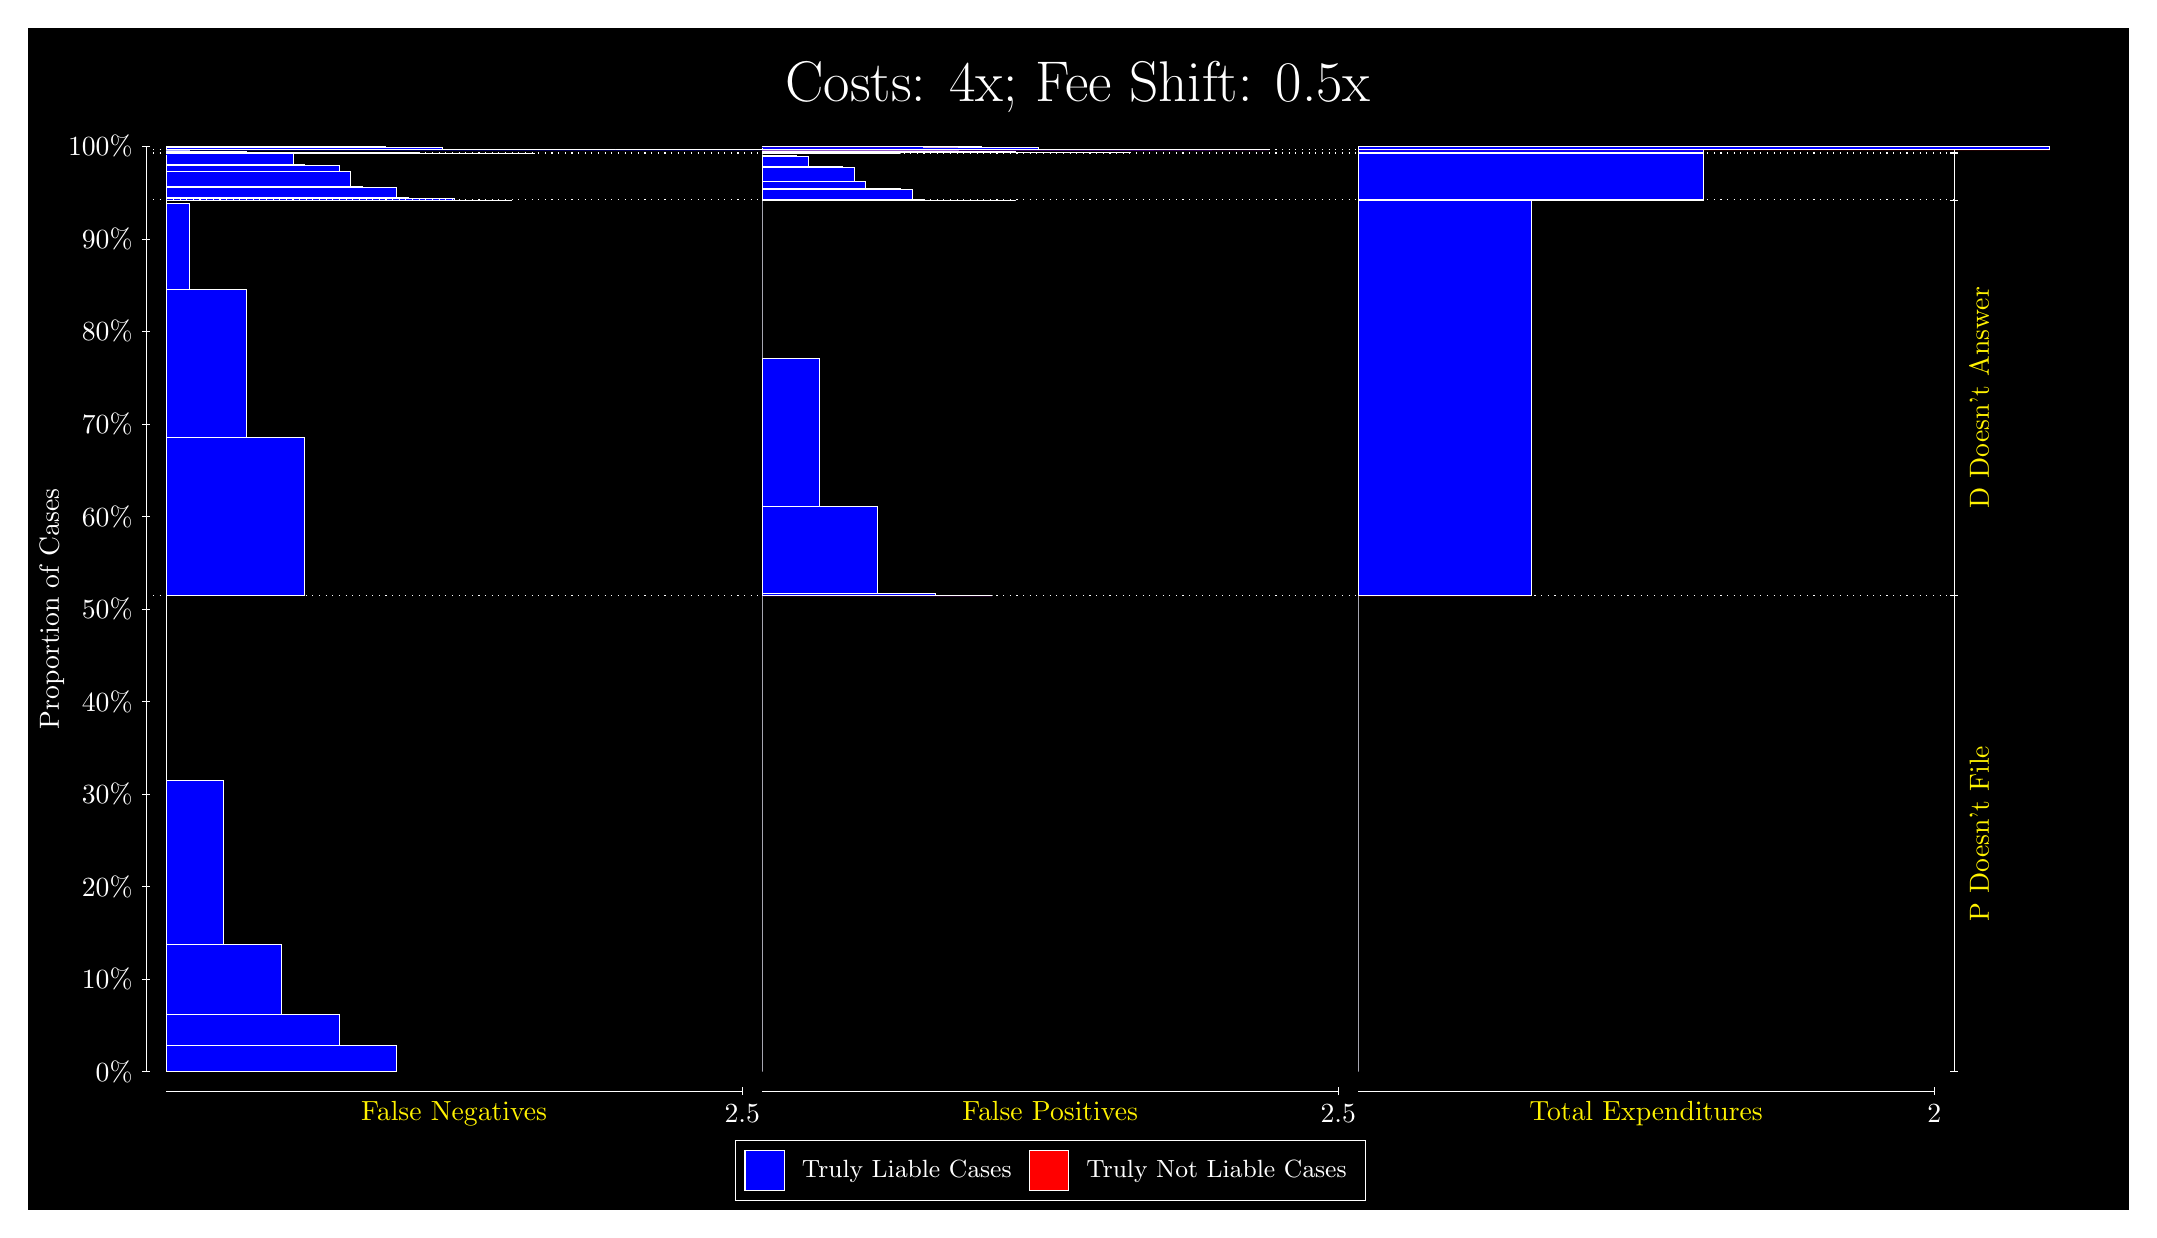
\begin{tikzpicture}
\draw[fill=black] (0,0) rectangle (26.667,15);
\draw[text=white] (0,13.5) rectangle (26.667,15) node[midway] {\huge Costs: 4x; Fee Shift: 0.5x};
\draw[white, very thin] (1.5,1.75) -- (1.5,13.5);
\node[rotate=90, text=white, anchor=center] at (0.3, 7.625) {Proportion of Cases};
\draw[white, very thin] (1.45,1.75) -- (1.55,1.75);
\node[text=white, anchor=east] at (1.45, 1.75) {0\%};
\draw[white, very thin] (1.45,2.925) -- (1.55,2.925);
\node[text=white, anchor=east] at (1.45, 2.925) {10\%};
\draw[white, very thin] (1.45,4.1) -- (1.55,4.1);
\node[text=white, anchor=east] at (1.45, 4.1) {20\%};
\draw[white, very thin] (1.45,5.275) -- (1.55,5.275);
\node[text=white, anchor=east] at (1.45, 5.275) {30\%};
\draw[white, very thin] (1.45,6.45) -- (1.55,6.45);
\node[text=white, anchor=east] at (1.45, 6.45) {40\%};
\draw[white, very thin] (1.45,7.625) -- (1.55,7.625);
\node[text=white, anchor=east] at (1.45, 7.625) {50\%};
\draw[white, very thin] (1.45,8.8) -- (1.55,8.8);
\node[text=white, anchor=east] at (1.45, 8.8) {60\%};
\draw[white, very thin] (1.45,9.975) -- (1.55,9.975);
\node[text=white, anchor=east] at (1.45, 9.975) {70\%};
\draw[white, very thin] (1.45,11.15) -- (1.55,11.15);
\node[text=white, anchor=east] at (1.45, 11.15) {80\%};
\draw[white, very thin] (1.45,12.325) -- (1.55,12.325);
\node[text=white, anchor=east] at (1.45, 12.325) {90\%};
\draw[white, very thin] (1.45,13.5) -- (1.55,13.5);
\node[text=white, anchor=east] at (1.45, 13.5) {100\%};

\draw[white, very thin] (24.457,1.75) -- (24.457,13.5);
\draw[white, very thin] (24.407,1.75) -- (24.507,1.75);
\node[anchor=west] at (24.407, 1.75) {};
\draw[white, very thin] (24.407,7.7923) -- (24.507,7.7923);
\node[anchor=west] at (24.407, 7.7923) {};
\draw[white, very thin] (24.407,12.819) -- (24.507,12.819);
\node[anchor=west] at (24.407, 12.819) {};
\draw[white, very thin] (24.407,13.409) -- (24.507,13.409);
\node[anchor=west] at (24.407, 13.409) {};
\draw[white, very thin] (24.407,13.425) -- (24.507,13.425);
\node[anchor=west] at (24.407, 13.425) {};
\draw[white, very thin] (24.407,13.457) -- (24.507,13.457);
\node[anchor=west] at (24.407, 13.457) {};
\draw[white, very thin] (24.407,13.5) -- (24.507,13.5);
\node[anchor=west] at (24.407, 13.5) {};

\draw[white, very thin, fill=blue] (1.75,1.75) rectangle (4.6775,2.0862);
\draw[white, very thin, fill=blue] (1.75,2.0862) rectangle (3.9457,2.4776);
\draw[white, very thin, fill=blue] (1.75,2.4776) rectangle (3.2138,3.3621);
\draw[white, very thin, fill=blue] (1.75,3.3621) rectangle (2.4819,5.445);
\draw[white, very thin, fill=red] (1.75,5.445) rectangle (1.75,5.445);
\draw[white, very thin, fill=blue] (1.75,5.445) rectangle (1.75,7.7923);
\draw[white, very thin, fill=blue] (1.75,7.7923) rectangle (3.5065,9.8051);
\draw[white, very thin, fill=blue] (1.75,9.8051) rectangle (2.7746,11.688);
\draw[white, very thin, fill=blue] (1.75,11.688) rectangle (2.0428,12.782);
\draw[white, very thin, fill=red] (1.75,12.782) rectangle (1.75,12.782);
\draw[white, very thin, fill=blue] (1.75,12.782) rectangle (1.75,12.819);
\draw[white, very thin, fill=blue] (1.75,12.819) rectangle (6.1413,12.819);
\draw[white, very thin, fill=blue] (1.75,12.819) rectangle (5.5558,12.82);
\draw[white, very thin, fill=blue] (1.75,12.82) rectangle (5.4094,12.838);
\draw[white, very thin, fill=blue] (1.75,12.838) rectangle (4.9703,12.838);
\draw[white, very thin, fill=blue] (1.75,12.838) rectangle (4.8239,12.857);
\draw[white, very thin, fill=blue] (1.75,12.857) rectangle (4.6775,12.984);
\draw[white, very thin, fill=blue] (1.75,12.984) rectangle (4.2384,12.991);
\draw[white, very thin, fill=blue] (1.75,12.991) rectangle (4.092,13.178);
\draw[white, very thin, fill=blue] (1.75,13.178) rectangle (3.9457,13.265);
\draw[white, very thin, fill=blue] (1.75,13.265) rectangle (3.5065,13.269);
\draw[white, very thin, fill=blue] (1.75,13.269) rectangle (3.3602,13.406);
\draw[white, very thin, fill=blue] (1.75,13.406) rectangle (3.2138,13.407);
\draw[white, very thin, fill=blue] (1.75,13.407) rectangle (2.7746,13.407);
\draw[white, very thin, fill=blue] (1.75,13.407) rectangle (2.6283,13.409);
\draw[white, very thin, fill=blue] (1.75,13.409) rectangle (2.0428,13.409);
\draw[white, very thin, fill=red] (1.75,13.409) rectangle (1.75,13.409);
\draw[white, very thin, fill=blue] (1.75,13.409) rectangle (6.4341,13.409);
\draw[white, very thin, fill=blue] (1.75,13.409) rectangle (5.7022,13.412);
\draw[white, very thin, fill=blue] (1.75,13.412) rectangle (4.9703,13.421);
\draw[white, very thin, fill=blue] (1.75,13.421) rectangle (4.2384,13.425);
\draw[white, very thin, fill=blue] (1.75,13.425) rectangle (3.5065,13.425);
\draw[white, very thin, fill=red] (1.75,13.425) rectangle (1.75,13.425);
\draw[white, very thin, fill=blue] (1.75,13.425) rectangle (3.5065,13.425);
\draw[white, very thin, fill=blue] (1.75,13.425) rectangle (2.7746,13.443);
\draw[white, very thin, fill=blue] (1.75,13.443) rectangle (2.0428,13.456);
\draw[white, very thin, fill=red] (1.75,13.456) rectangle (1.75,13.456);
\draw[white, very thin, fill=blue] (1.75,13.456) rectangle (1.75,13.457);
\draw[white, very thin, fill=blue] (1.75,13.457) rectangle (9.9471,13.457);
\draw[white, very thin, fill=blue] (1.75,13.457) rectangle (9.2152,13.457);
\draw[white, very thin, fill=blue] (1.75,13.457) rectangle (8.4834,13.457);
\draw[white, very thin, fill=blue] (1.75,13.457) rectangle (7.7515,13.46);
\draw[white, very thin, fill=blue] (1.75,13.46) rectangle (7.4587,13.46);
\draw[white, very thin, fill=blue] (1.75,13.46) rectangle (7.0196,13.46);
\draw[white, very thin, fill=blue] (1.75,13.46) rectangle (6.7268,13.46);
\draw[white, very thin, fill=blue] (1.75,13.46) rectangle (6.2877,13.46);
\draw[white, very thin, fill=blue] (1.75,13.46) rectangle (5.9949,13.468);
\draw[white, very thin, fill=blue] (1.75,13.468) rectangle (5.2631,13.489);
\draw[white, very thin, fill=blue] (1.75,13.489) rectangle (4.5312,13.499);
\draw[white, very thin, fill=blue] (1.75,13.499) rectangle (3.7993,13.5);
\draw[white, very thin, fill=blue] (1.75,13.5) rectangle (3.0674,13.5);
\draw[white, very thin, fill=blue] (1.75,13.5) rectangle (2.3355,13.5);
\draw[white, very thin, fill=red] (1.75,13.5) rectangle (1.75,13.5);
\draw[white, very thin, fill=red] (9.3189,1.75) rectangle (9.3189,1.75);
\draw[white, very thin, fill=blue] (9.3189,1.75) rectangle (9.3189,7.7923);
\draw[white, very thin, fill=red] (9.3189,7.7923) rectangle (12.246,7.7923);
\draw[white, very thin, fill=blue] (9.3189,7.7923) rectangle (12.246,7.7923);
\draw[white, very thin, fill=blue] (9.3189,7.7923) rectangle (11.515,7.8301);
\draw[white, very thin, fill=blue] (9.3189,7.8301) rectangle (10.783,8.9233);
\draw[white, very thin, fill=blue] (9.3189,8.9233) rectangle (10.051,10.807);
\draw[white, very thin, fill=blue] (9.3189,10.807) rectangle (9.3189,12.819);
\draw[white, very thin, fill=red] (9.3189,12.819) rectangle (12.539,12.819);
\draw[white, very thin, fill=blue] (9.3189,12.819) rectangle (12.539,12.819);
\draw[white, very thin, fill=red] (9.3189,12.819) rectangle (11.954,12.819);
\draw[white, very thin, fill=blue] (9.3189,12.819) rectangle (11.954,12.821);
\draw[white, very thin, fill=blue] (9.3189,12.821) rectangle (11.807,12.821);
\draw[white, very thin, fill=red] (9.3189,12.821) rectangle (11.368,12.821);
\draw[white, very thin, fill=blue] (9.3189,12.821) rectangle (11.368,12.822);
\draw[white, very thin, fill=blue] (9.3189,12.822) rectangle (11.222,12.959);
\draw[white, very thin, fill=blue] (9.3189,12.959) rectangle (11.075,12.963);
\draw[white, very thin, fill=blue] (9.3189,12.963) rectangle (10.636,13.05);
\draw[white, very thin, fill=blue] (9.3189,13.05) rectangle (10.49,13.237);
\draw[white, very thin, fill=blue] (9.3189,13.237) rectangle (10.344,13.244);
\draw[white, very thin, fill=blue] (9.3189,13.244) rectangle (9.9044,13.371);
\draw[white, very thin, fill=blue] (9.3189,13.371) rectangle (9.758,13.39);
\draw[white, very thin, fill=blue] (9.3189,13.39) rectangle (9.6116,13.39);
\draw[white, very thin, fill=blue] (9.3189,13.39) rectangle (9.3189,13.409);
\draw[white, very thin, fill=red] (9.3189,13.409) rectangle (11.075,13.409);
\draw[white, very thin, fill=blue] (9.3189,13.409) rectangle (11.075,13.409);
\draw[white, very thin, fill=blue] (9.3189,13.409) rectangle (10.344,13.413);
\draw[white, very thin, fill=blue] (9.3189,13.413) rectangle (9.6116,13.422);
\draw[white, very thin, fill=blue] (9.3189,13.422) rectangle (9.3189,13.425);
\draw[white, very thin, fill=red] (9.3189,13.425) rectangle (14.003,13.425);
\draw[white, very thin, fill=blue] (9.3189,13.425) rectangle (14.003,13.425);
\draw[white, very thin, fill=blue] (9.3189,13.425) rectangle (13.271,13.425);
\draw[white, very thin, fill=blue] (9.3189,13.425) rectangle (12.539,13.439);
\draw[white, very thin, fill=blue] (9.3189,13.439) rectangle (11.807,13.456);
\draw[white, very thin, fill=blue] (9.3189,13.456) rectangle (11.075,13.457);
\draw[white, very thin, fill=red] (9.3189,13.457) rectangle (15.759,13.457);
\draw[white, very thin, fill=blue] (9.3189,13.457) rectangle (15.759,13.457);
\draw[white, very thin, fill=blue] (9.3189,13.457) rectangle (15.028,13.457);
\draw[white, very thin, fill=red] (9.3189,13.457) rectangle (15.028,13.457);
\draw[white, very thin, fill=blue] (9.3189,13.457) rectangle (15.028,13.457);
\draw[white, very thin, fill=blue] (9.3189,13.457) rectangle (14.296,13.457);
\draw[white, very thin, fill=red] (9.3189,13.457) rectangle (14.296,13.457);
\draw[white, very thin, fill=blue] (9.3189,13.457) rectangle (14.296,13.457);
\draw[white, very thin, fill=blue] (9.3189,13.457) rectangle (13.564,13.46);
\draw[white, very thin, fill=red] (9.3189,13.46) rectangle (13.564,13.46);
\draw[white, very thin, fill=blue] (9.3189,13.46) rectangle (13.564,13.467);
\draw[white, very thin, fill=blue] (9.3189,13.467) rectangle (12.832,13.467);
\draw[white, very thin, fill=blue] (9.3189,13.467) rectangle (12.832,13.489);
\draw[white, very thin, fill=blue] (9.3189,13.489) rectangle (12.1,13.496);
\draw[white, very thin, fill=red] (9.3189,13.496) rectangle (11.807,13.496);
\draw[white, very thin, fill=blue] (9.3189,13.496) rectangle (11.807,13.496);
\draw[white, very thin, fill=blue] (9.3189,13.496) rectangle (11.368,13.497);
\draw[white, very thin, fill=red] (9.3189,13.497) rectangle (11.075,13.497);
\draw[white, very thin, fill=blue] (9.3189,13.497) rectangle (11.075,13.497);
\draw[white, very thin, fill=blue] (9.3189,13.497) rectangle (10.636,13.497);
\draw[white, very thin, fill=blue] (9.3189,13.497) rectangle (10.344,13.499);
\draw[white, very thin, fill=blue] (9.3189,13.499) rectangle (9.6116,13.5);
\draw[white, very thin, fill=blue] (9.3189,13.5) rectangle (9.3189,13.5);
\draw[white, very thin, fill=red] (16.888,1.75) rectangle (16.888,1.75);
\draw[white, very thin, fill=blue] (16.888,1.75) rectangle (16.888,7.7923);
\draw[white, very thin, fill=red] (16.888,7.7923) rectangle (19.083,7.7923);
\draw[white, very thin, fill=blue] (16.888,7.7923) rectangle (19.083,12.819);
\draw[white, very thin, fill=red] (16.888,12.819) rectangle (21.279,12.819);
\draw[white, very thin, fill=blue] (16.888,12.819) rectangle (21.279,12.83);
\draw[white, very thin, fill=red] (16.888,12.83) rectangle (21.279,12.83);
\draw[white, very thin, fill=blue] (16.888,12.83) rectangle (21.279,13.409);
\draw[white, very thin, fill=red] (16.888,13.409) rectangle (21.279,13.409);
\draw[white, very thin, fill=blue] (16.888,13.409) rectangle (21.279,13.425);
\draw[white, very thin, fill=red] (16.888,13.425) rectangle (21.279,13.425);
\draw[white, very thin, fill=blue] (16.888,13.425) rectangle (21.279,13.457);
\draw[white, very thin, fill=red] (16.888,13.457) rectangle (25.67,13.457);
\draw[white, very thin, fill=blue] (16.888,13.457) rectangle (25.67,13.46);
\draw[white, very thin, fill=red] (16.888,13.46) rectangle (25.67,13.46);
\draw[white, very thin, fill=blue] (16.888,13.46) rectangle (25.67,13.5);
\draw[white, dotted] (1.5,7.7923) -- (24.457,7.7923);
\draw[white, dotted] (1.5,12.819) -- (24.457,12.819);
\draw[white, dotted] (1.5,13.409) -- (24.457,13.409);
\draw[white, dotted] (1.5,13.425) -- (24.457,13.425);
\draw[white, dotted] (1.5,13.457) -- (24.457,13.457);
\draw[white, very thin] (1.75,1.5) -- (9.0689,1.5);
\node[text=yellow, anchor=north] at (5.4094, 1.5) {False Negatives};
\draw[white, very thin] (9.0689,1.45) -- (9.0689,1.55);
\node[text=white, anchor=north] at (9.0689, 1.45) {2.5};

\draw[white, very thin] (9.3189,1.5) -- (16.638,1.5);
\node[text=yellow, anchor=north] at (12.978, 1.5) {False Positives};
\draw[white, very thin] (16.638,1.45) -- (16.638,1.55);
\node[text=white, anchor=north] at (16.638, 1.45) {2.5};

\draw[white, very thin] (16.888,1.5) -- (24.207,1.5);
\node[text=yellow, anchor=north] at (20.547, 1.5) {Total Expenditures};
\draw[white, very thin] (24.207,1.45) -- (24.207,1.55);
\node[text=white, anchor=north] at (24.207, 1.45) {2};

\node[text=yellow, centered, rotate=90] at (24.777, 4.7711) {P Doesn't File};
\node[text=yellow, centered, rotate=90] at (24.777, 10.306) {D Doesn't Answer};





\draw (12.978300999999998,1.5) node[draw=none] (baseCoordinate) {};
\begin{scope}[align=center]
        \matrix[scale=0.5, draw=white, below=0.5cm of baseCoordinate, nodes={draw}, column sep=0.1cm]{
            \node[rectangle, draw, minimum width=0.5cm, minimum height=0.5cm, fill=blue] {}; &
            \node[draw=none, font=\small, text=white] (B) {Truly Liable Cases}; &
            \node[rectangle, draw, minimum width=0.5cm, minimum height=0.5cm, fill=red] {}; &
            \node[draw=none, font=\small, text=white] (B) {Truly Not Liable Cases}; \\
            };
\end{scope}

\end{tikzpicture}
\end{document}